\newcommand{\answerA}[5]{
\section{#1}

\noindent
{\textbf{Przykładowa odpowiedź:}}
#2
\textbf{\ifstrequal{#3}{T}{PRAWDA}{
    \ifstrequal{#3}{F}{FAŁSZ}{DIY}
}}

\vspace{0.4cm}
\noindent
\textbf{Odpowiedź:}
#4

\vspace{0.4cm}
\noindent
\textbf{Wyjaśnienie:} 
#5
}

\newcommand{\answerB}[4]{
\section{#1}

\noindent
{\textbf{Przykładowa odpowiedź:}}
#2
\textbf{\ifstrequal{#3}{T}{PRAWDA}{
    \ifstrequal{#3}{F}{FAŁSZ}{DIY}
}}

\vspace{0.4cm}
\noindent
\textbf{Odpowiedź:}
#4
}

\newcommand{\answerC}[4]{
\section{#1}

\noindent
{\textbf{Przykładowa odpowiedź:}}
#2
\textbf{\ifstrequal{#3}{T}{PRAWDA}{
    \ifstrequal{#3}{F}{FAŁSZ}{DIY}
}}

\vspace{0.4cm}
\noindent
\textbf{Wyjaśnienie:} 
#4
}

\chapter{Programowanie współbieżne i~rozproszone}
\PartialToc

\answerA
{Jak wygląda poprawna definicja obiektu funkcyjnego w języku Erlang?}
{F1 = fun (X) -> X + 1 end.}
{T}
{Ogólna postać to F = fun(paramtery) -> ciało end.}
{Obiekt funkcyjny - fun() - jest~jednym z~typów danych w~Erlangu, umożliwia stworzenie funkcji anonimowej, która~będzie w~sobie zawierała odwołanie do~prawdziwej funkcji.}

\answerA
{Jaki będzie wynik operacji w Erlangu: [1,2,3] -- -- [3,2,3,5]?}
{[1]}
{T}
{[1]}
{Operator ''-- --'' najpierw tworzy kopie tablicy będącej jego pierwszym argumentem, a~następnie dla~każdego elementu z~drugiej tablicy usuwa pierwsze wystąpienie (jeżeli w~ogóle takie istnieje) tego elementu w~pierwszej tablicy np. dla~wywołania [1,2,3,2,1,2] -- -- [2,1,2] zwrócone zostanie [3,1,2].}

\answerA
{System typów w Erlangu jest:}
{Dynamiczny - sprawdzany w trakcie kompilacji}
{F}
{Erlang jest językiem z~dynamicznym, silnym typowaniem.}
{\\}
\noindent
\textbf{Typowanie dynamiczne} - przypisywanie typów do~wartości przechowywanych w~zmiennych w~trakcie działania programu. Przy zastosowaniu typowania dynamicznego, zmienne nie~posiadają typów przypisanych statycznie, czyli przed uruchomieniem programu np.~w~trakcie kompilacji. W~takiej sytuacji typ~zmiennej wynika z~wartości jaką dana zmienna przechowuje. Jest to~jeden ze~sposobów na~zwolnienie programisty z~obowiązku deklarowania typów zmiennych.
\noindent
\textbf{Silna typizacja} – każde wyrażenie ma~ustalony typ i~nie~można go~używać w~kontekście przeznaczonym dla~innych typów.
\begin{lstlisting}[language=C]
int liczba = 1;
if ("1" == liczba) { ... }
\end{lstlisting}
W powyższym kodzie nastąpi błąd podczas kompilacji, ponieważ ''1'' to~typ tekstowy (string), zatem nie~jest liczbą (int).

\answerA
{W jaki sposób tworzy się proces w języku Erlang wykonujący funkcję F1?}
{Pid is spawn\_exec(F1)}
{F}
{Pid = spawn(F1)}
{Procesy tworzy się przy użyciu funkcji spawn, która w~swojej najprostrzej postaci przyjmuje tylko jeden argument będący funkcją (tą, którą nowo powstały proces ma~wykonywać) i~zwraca Pid utworzonego procesu.}

\answerA
{Jak w języku Erlang wysyła się wiadomość (Mesg) do procesu posiadając jego identyfikator (Pid)?}
{retVal = send(Pid, Mesg)}
{F}
{Pid ! Mesg.}
{Wiadomości wysyła przy użyciu operatora ''!''.}

\answerB
{Jaki model jest użyty do komunikacji między procesami w języku Erlang?}
{Model pamięci współdzielonej}
{F}
{Erlang używa modelu aktora, gdzie aktorzy (odseparowane od~siebie procesy na~wirtualnej maszynie Erlanga) komunikują się~ze~sobą przesyłając sobie wiadomości (model przesyłania komunikatów).}

\answerB
{Jak realizowana jest komunikacja między procesami w języku Erlang?}
{Jest oparta na spotkaniach}
{F}
{Procesy wysyłają sobie wiadomości (komunikacja asynchroniczna)}

\answerA
{Jaki będzie wynik wykonania następującej instrukcji w języku Erlang: lists:map(fun(X) -> \{X,X+1\} end, [1,2,3])?}
{\{\{1,2\},\{2,3\},\{3,4\}\}}
{F}
{[\{1,2\},\{2,3\},\{3,4\}]}
{Pierwszym argumentem map'a jest~funkcja, która zostanie zaaplikowana do~każdego elementu listy będącej drugiem argumentem funkcji map, zwrócona zostaje lista wyników wywołania. W~powyższym przypadku zwrócona zostanie lista krotek postaci \{X,X+1\}, gdzie za~X wstawiane będą kolejno 1,2,3.}

\answerC
{Jaka jest funkcja obiektu chronionego w Adzie?}
{Kontroluje dostęp do współdzielonych danych}
{T}
{Obiekt chroniony jest jednostką programową, która~organizuje dostęp zadań do~grupowanych przez siebie danych współdzielonych. Jest odpowiednikiem \underline{monitora}. Obiekt chroniony stosujemy, gdy~chcemy współbieżnie dzielić się~zasobami, a~zależy nam~na~bezpieczeństwie, by~w~czasie zmieniania współdzielonej wartości nie~odczytywać niegotowej zmiennej. W~obiekcie chronionym modyfikacje mogą przeprowadzać tylko procedury. Oprócz nich dostępne są~jeszcze funkcje i~wejścia (które z~kolei mogą posiadać bariery).}

\newpage

\answerA
{Jakie operacje są możliwe do zdefiniowania dla typu kontrolowanego w Adzie?}
{Tylko operator przypisania}
{F}
{Inicjalizacja po~stworzeniu, finalizacja przed~unicestwieniem, poprawka po~przypisaniu}
{Podstawowe operacje dla~typu kontrolowanego \emph{(Ada.Finalization.Controlled)}:
\begin{itemize}
\item \textbf{initialize} inicjalizacja po~stworzeniu, co~daje nam możliwość wykonania danej procedury zaraz po~utworzeniu zmiennej typu kontrolowanego,
\item \textbf{finalize} finalizacja przed~unicestwieniem, analogicznie jak~wyżej, jednak przy~pozbywaniu się~zmiennej,
\item \textbf{adjust} poprawka po~przypisaniu, czyli w~momencie zmiany wartości kontrolowanej zmiennej, możemy wykonać zdefiniowane działanie.
\end{itemize}}

\answerB
{W jaki sposób określa się kierunek przekazywania argumentów z/do procedur w języku Ada?}
{Symbole -> oraz <- w deklaracji parametrów}
{F}
{Kierunek przekazywania argumentów możana określić wpisując przed~typem parametru czy~dany parametr ma~być wejściowy (in), wyjściowy (out) czy~jedno i~drugie (in~out). Domyślnie każdy parametr jest~wejściowy. Przykład: procedure JakasProcedura(A, B : in out Float; C : Float); W~przypadku C~parametr domyślnie jest~wejściowy.}

\answerA
{Jaki jest rodzaj typizacji w języku Ada?}
{opcjonalny}
{F}
{Ada jest językiem o statycznej, silnej typizacji.}
{\\
\textbf{Typowanie statyczne} – nadawanie typów zmiennym w~czasie kompilacji programu. W~porównaniu do~typowania dynamicznego, zaletami są~możliwość większej optymalizacji oraz~możliwość wykrycia większej liczby błędów w~czasie kompilacji. Wadą jest~natomiast konieczność pisania dużej ilości informacji o~typach. \\
\textbf{Silna typizacja} została opisana w~jednym z~powyższych pytań.}

\answerB
{Jak komunikują się zadania w jezyku Ada?}
{Przez przesyłanie wiadomości}
{F}
{Zadania w języku Ada komunikują się~przez~tzw.~spotkania albo~randki. W~spotkaniu uczestniczą dwa (lub~więcej) procesy (nazywane w~Adzie zadaniami). Oprócz spotkań (randek) istnieją jeszcze obiekty chronione i~zmienne dzielone będące~niejako wspólnym źródłem danych, spotkania natomiast są~trochę bardziej skomplikowane, gdyż~umożliwiają interakcję.}

\answerB
{Które z wymienionych algorytmów służą do wyboru lidera w systemie rozproszonym?}
{Algorytm Amdahla}
{F}
{Algorytmy elekcji (wyboru lidera) w~systemie rozproszonym:
\begin{itemize}

\item algorytm tyrana (bully algorithm). Po~otrzymaniu komunikatu elekcji lub~po~wykryciu braku koordynatora, proces rozsyła komunikat elekcji do~wszystkich procesów, które mają~wyższy priorytet od~niego. W~momencie, gdy~proces nie~otrzyma odpowiedzi od~żadnego z~procesów o~wyższym priorytecie od~jego własnego, wtedy rozsyła komunikat do~wszystkich, że~został nowym koordynatorem.

\begin{center}
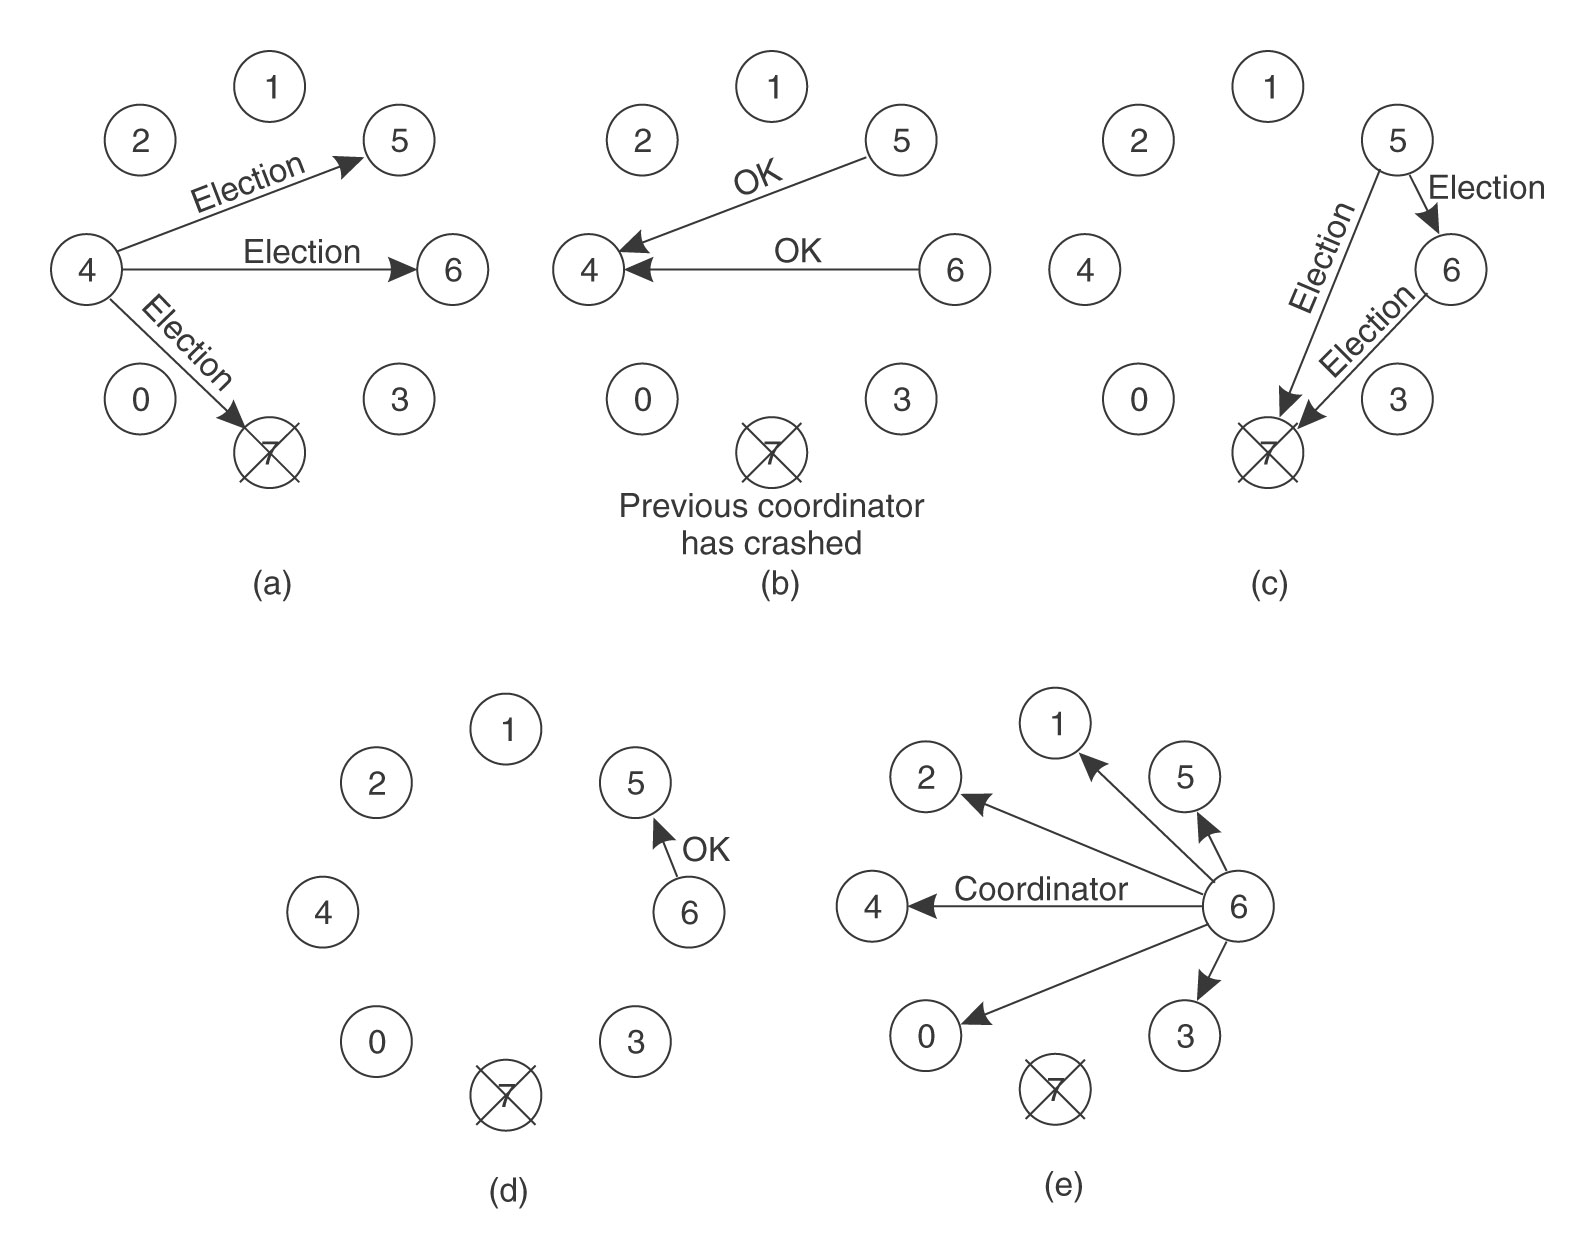
\includegraphics[width=16.5cm]{16/tyran}
\captionof{figure}{Algorytm tyrana}
\end{center}

\item algorytm pierścieniowy (ring algorithm):
    \begin{itemize}
    \item według Tanenbauma
        \begin{center}
        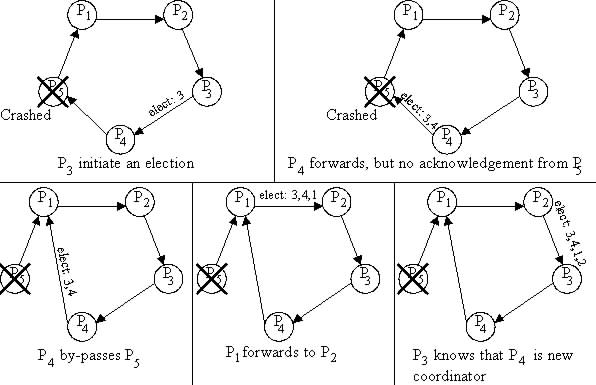
\includegraphics[width=15cm]{16/ring}
        \captionof{figure}{Algorytm pierścieniowy według Tanenbauma}
        \end{center}
            Poniższy rysunek obrazuje działanie algorytmu w~przypadku, gdy~dwa procesy (2~i~5) odkryły, że~koordynator nie~działa i~rozpoczęły dwie równoczesne elekcje.
    
        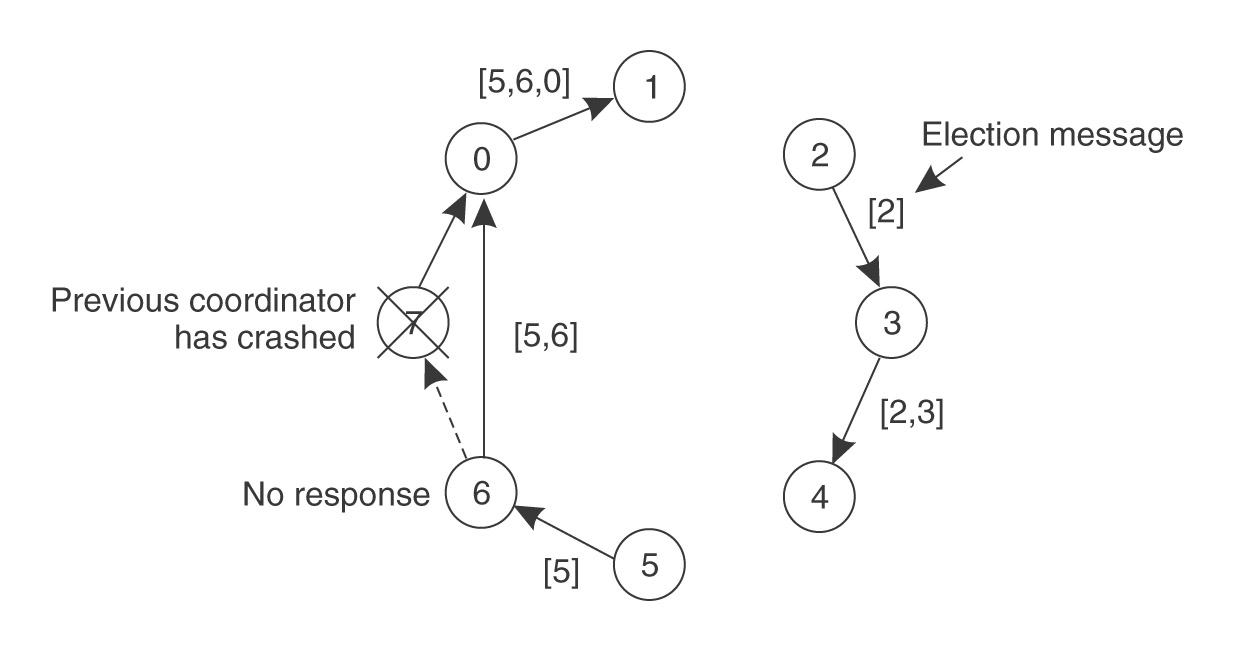
\includegraphics[width=12cm]{16/ring_double_election}
    
    \item według Coulourisa (nie był omawiany przez PTMa)
    
        Aby uniknąć powielania elekcji tak jak w~Tannenbaumie, algorytm Coulourisa wprowadza dodatkową flagę w~każdym z~procesów, która informuje czy~dany proces uczestniczy w~danej chwili w~elekcji.
    
    \end{itemize}
\end{itemize}}

\newpage

\answerC
{Zaznacz prawdziwe zdania}
{Prawo Amdahla pozwala oszacować \underline{teoretyczny} wzrost szybkości systemu przy~zmianie liczby procesorów}
{T}
{\underline{W teorii} prawo Amdahla jest w~stanie oszacować maksymalny wzrost, ale \underline{w~praktyce} wychodzi to~zdecydowanie gorzej.

\noindent
Prawo Amdahla jest używane do~znajdowania maksymalnego spodziewanego zwiększenia wydajności całkowitej systemu jeżeli tylko~część systemu została ulepszona. Jest ono~często używane w~przypadku prowadzenia obliczeń równoległych do~przewidzenia teoretycznego maksymalnego wzrostu szybkości obliczeń przy~użyciu wielu procesorów.

\noindent
Zwiększenie szybkości wykonywania się programu przy~użyciu wielu procesorów w~obliczeniach równoległych jest ograniczane przez~czas potrzebny do~sekwencyjnego dzielenia programu. Na~przykład jeżeli program potrzebuje 20~godzin w~przypadku obliczeń prowadzonych na~procesorze jednordzeniowym i~1~godzina obliczeń nie~może zostać przetworzona poprzez obliczenia równoległe, ale~pozostałe 19 godzin (95\%) obliczeń mogą, wówczas bez~względu na~to~ile~procesorów zostanie użytych do~przeprowadzenia obliczeń równoległych minimalny czas wykonania programu nie~będzie nigdy mniejszy niż~ta~krytyczna 1~godzina. Tak więc zwiększenie szybkości obliczeń jest ograniczone do~20x, jak przedstawiono na~poniższym diagramie:

\begin{center}
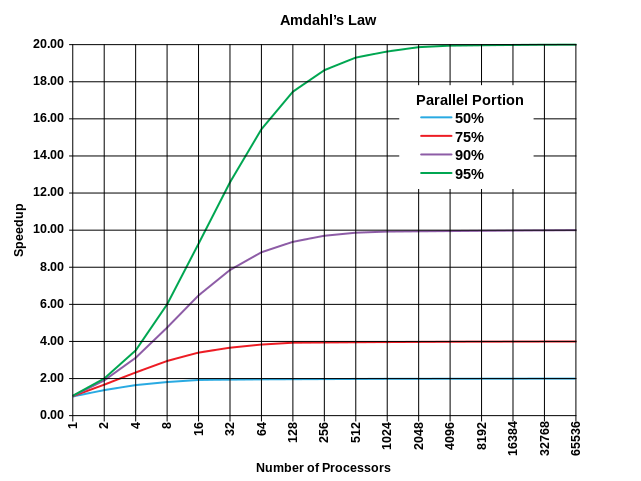
\includegraphics[width=14cm]{16/amdahl}
\captionof{figure}{Prawo Amdahla}
\end{center}}